% Source : http://melusine.eu.org/syracuse/wiki/doku.php/pgf/tikz/index

\documentclass{article}
	\usepackage{fourier}
	\usepackage{pgfplots}

	\pagestyle{empty}


\begin{document}

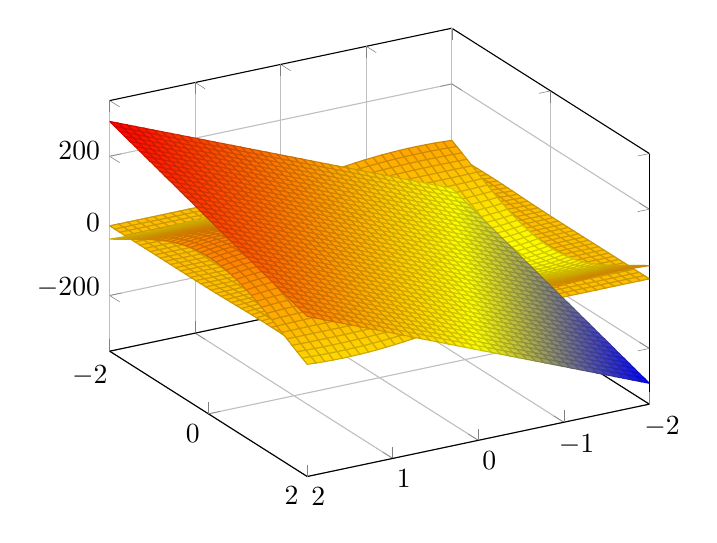
\begin{tikzpicture}
	\begin{axis}[grid=major,view={150}{30}]
		\addplot3[surf,shader=faceted,samples=40,domain=-2:2,y domain=-2:2]%
		{100*sin(deg(x))*sin(deg(y))*exp(-x*x+x*y-y*y)};

		\addplot3[surf,shader=faceted,samples=40,domain=-2:2,y domain=-2:2]%
		{100*sin(deg(x))*cos(deg(y))};

		\addplot3[surf,shader=faceted,samples=40,domain=-2:2,y domain=-2:2]%
		{100*x-50*y};
	\end{axis}
\end{tikzpicture}

\end{document}
